\documentclass[10pt]{beamer}
\usepackage[utf8]{inputenc}
\usepackage{hyperref}
\usepackage[scaled]{helvet}
\usepackage[T1]{fontenc}
\usetheme{Berkeley}
\beamertemplatenavigationsymbolsempty
\setbeamertemplate{headline}{}
\setbeamersize{sidebar width left=1.5cm}
\setbeamerfont{section in sidebar}{size=\fontsize{6}{6}\selectfont}
\setbeamerfont{title in sidebar}{size=\fontsize{6}{6}\selectfont}
%https://github.com/SiLeBAT/BfROpenLabResources/raw/master/GitHubPages/documents/foodchainlab_import/
\title{Import FoodChain-Lab Workflow}
\date{}

\begin{document}
\maketitle

\section{1}
\begin{frame}
	\begin{center}
  		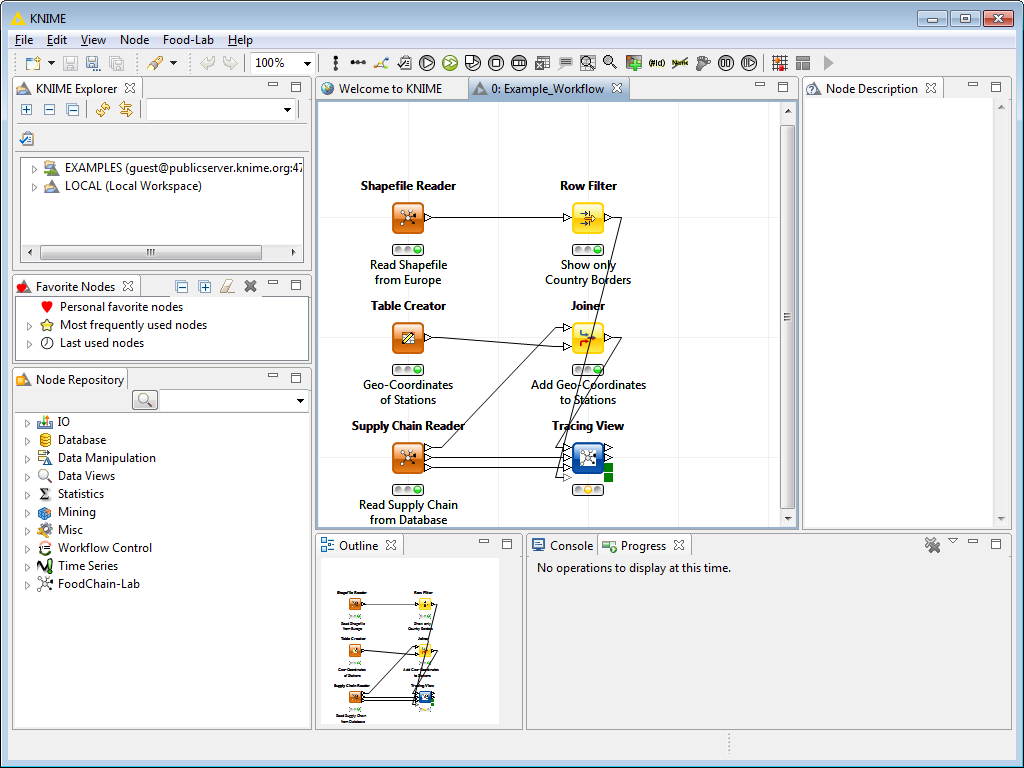
\includegraphics[height=0.6\textheight]{https://github.com/SiLeBAT/BfROpenLabResources/raw/master/GitHubPages/documents/foodchainlab_import/1.png}
	\end{center}
	\begin{itemize}
		\item Download the workflow you would like to import, e.g.
    \url{https://github.com/SiLeBAT/BfROpenLabResources/raw/master/GitHubPages/workflows/FCL_Example.zip}
		\item Right click on \textbf{LOCAL} in the \textbf{KNIME Explorer} view and select \textbf{Import KNIME Workflow}.
	\end{itemize}
\end{frame}

\section{2}
\begin{frame}
	\begin{center}
  		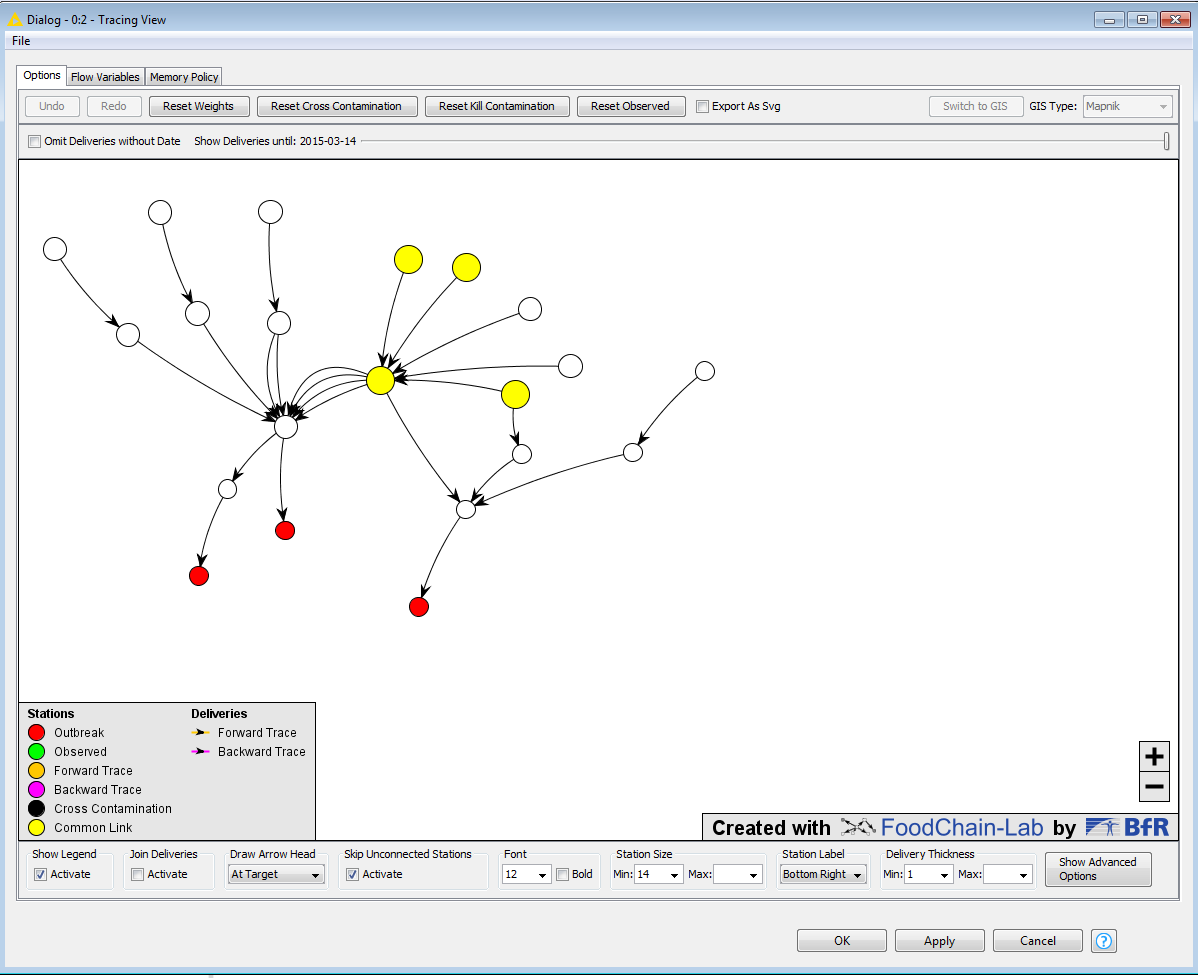
\includegraphics[height=0.6\textheight]{https://github.com/SiLeBAT/BfROpenLabResources/raw/master/GitHubPages/documents/foodchainlab_import/2.png}
	\end{center}
	\begin{itemize}
		\item In the import dialog choose \textbf{Select file} and click the \textbf{Browse} button.
	\end{itemize}
\end{frame}

\section{3}
\begin{frame}
	\begin{center}
  		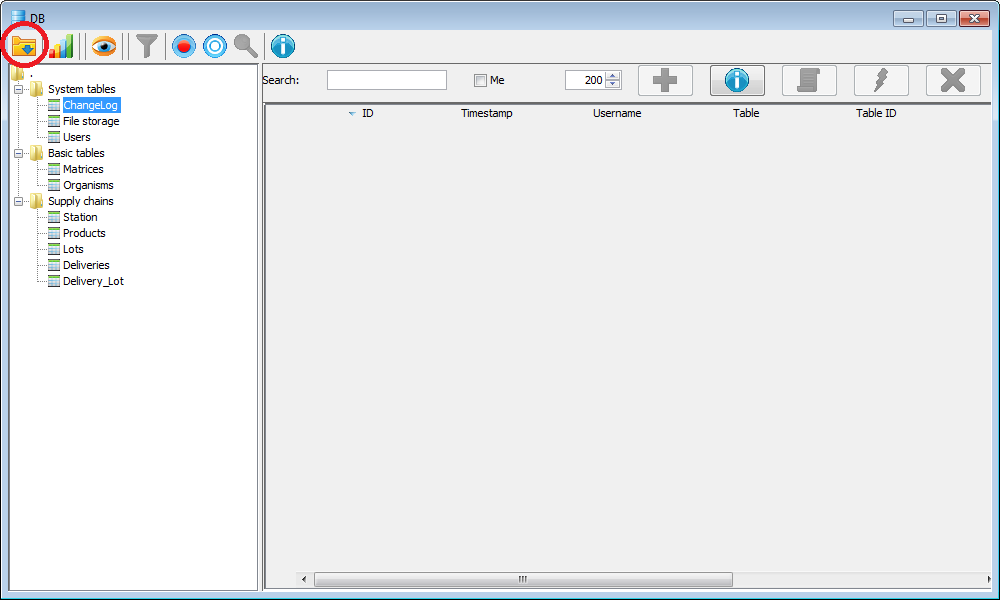
\includegraphics[height=0.6\textheight]{https://github.com/SiLeBAT/BfROpenLabResources/raw/master/GitHubPages/documents/foodchainlab_import/3.png}
	\end{center}
	\begin{itemize}
		\item Select the downloaded zipped workflow and Click \textbf{Open}.
	\end{itemize}
\end{frame}

\section{4}
\begin{frame}
	\begin{center}
  		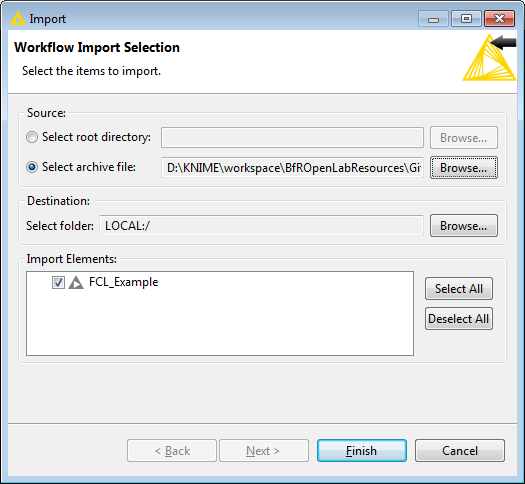
\includegraphics[height=0.6\textheight]{https://github.com/SiLeBAT/BfROpenLabResources/raw/master/GitHubPages/documents/foodchainlab_import/4.png}
	\end{center}
	\begin{itemize}
		\item In the Import dialog, you'll see the selected workflow.
		\item Click \textbf{Finish}.
	\end{itemize}
\end{frame}

\section{5}
\begin{frame}
	\begin{center}
  		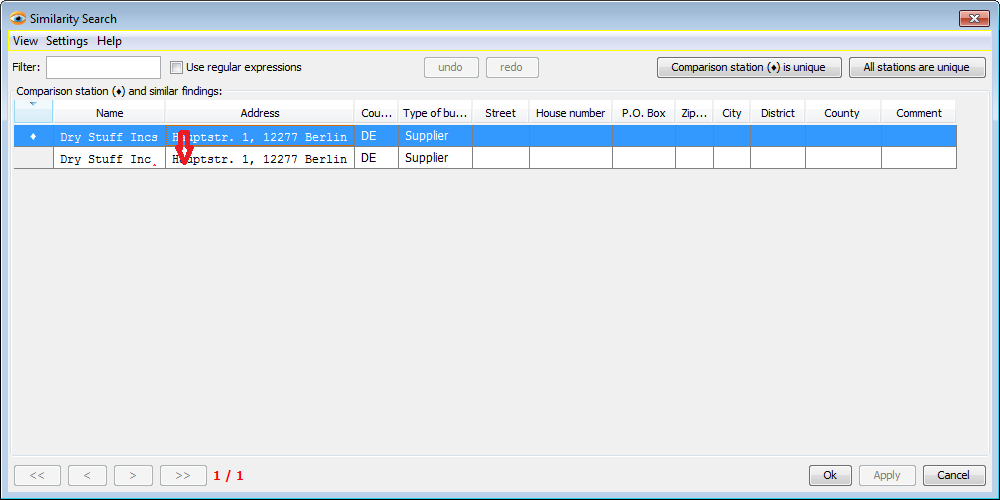
\includegraphics[height=0.6\textheight]{https://github.com/SiLeBAT/BfROpenLabResources/raw/master/GitHubPages/documents/foodchainlab_import/5.png}
	\end{center}
	\begin{itemize}
		\item In the KNIME workbench, expand \textbf{LOCAL} in the \textbf{KNIME Explorer} view and double click on the imported workflow.
		\item The workflow should show up in the Workflow Editor now (see red square).
	\end{itemize}
\end{frame}

\end{document}
